\chapter{Synchronization of Database Content}

\section{Definition of Terms}

Before presenting the basic principles of synchronization of animal
biodiversity databases some terms need to be defined.

\begin{itemize}
\item The smallest synchronization item will be referred as {}``data element''. 
\item Each database that is part of the global information system will be
called {}``node''.
\item Each node that provides new data element to the network is {}``owner''
of this data element.
\item {}``Representative'' of the owner is a node that can distribute
owners data. The representative has to have one to one relationship
to owner or to other representative of this owner. Representative
can be only node that needs this data, therefore there will be no
nodes that serve as buffers or transporters for data.
\item {}``Source'' - any node that distributes data elements to other
nodes is {}``source'' for this data elements for that nodes
\item {}``Target'' is the set of nodes to which one source distribute
a data element
\item {}``Network manager'' - the management authority that will route
the traffic of information, preventing conflicts or inconsistencies
\end{itemize}

\section{Synchronization Requirements}

We define the following list of features and constraints that we consider
appropriate for the intended use in EFABIS or APIIS:

\begin{enumerate}
\item Each data element has one and only one owner. Only the owner can modify
the data element.\\
In animal breeding information systems, data is usually collected
on different places - like AI stations, farms, research institutes.
The common of all these sources of information is that they keep copy
of data, there is somebody (human or organisation) that is officially
responsible for the quality of data and all users of this data rely
on its representative value. Therefore the definition of the term
{}``owner'' will be expanded as {}``member of the Information System
who is presenting data to the information space and is responsible
for its accuracy and up-to-date status''. For example each national
node in EFABIS that presents its country data to the European(EAAP)
and global (FAO) node is owner of this data and is responsible for
the data quality.
\item Each data element has a {}``distribution target'' or just {}``target''.\\
In general terms, the data collection process does not end in itself.
Usually the collected data is intended to be used by someone and in
most cases the data users are clearly defined. For example data collected
on testing stations is sent to research institute for calculating
the breeding values and the results are returned to the farmers.Or
in EFABIS network each European country will send data to EAAP and
EAAP will distribute this data to FAO. Therefore for each data element
there is a well defined target group of consumers. This list of users
is actually covered by the {}``distribution target''. This list
can consist of one or more addresses of nodes, these are the nodes
to which this data item will be distributed. If the distribution target
is an empty list then this element is only for private use and will
not be distributed.
\item Distribution target may be freely changed if this will not produce
inconsistencies.\\
This principle ensures that owner can freely choose target nodes unless
this will disturb normal floating of data in the system. All actions
have to be coordinated by the Network manager described in principle
7.
\item Synchronizations cannot be refused.\\
When a session is started it automatically synchronizes all of the
target content, thus do not allowing the user to refuse receiving
of changes. This principle may look very restricting and leaving no
choice to the users but it is not the case. The idea behind is that
user who wants to have this data element is accepting by default all
changes made by owner relying on the fact that all owner changes are
representative. For example if owner deletes one data element then
this element should be deleted everywhere. This is the situation in
EFABIS where only the country can edit its data.
\item All information to be transfered between nodes is considered element
of the synchronization process.\\
This principle states that we will not only synchronize data fields
in the database containing quantitative values like size, milk, wool
length, but also documents and multimedia data. This may look obvious,
but it is important for the type and quantity of the data that will
be transmitted.
\item For one data element only one source is allowed.\\
This source could be any node that has (and needs) this data element. \\
If the user node can establish connection to more than one representative
then the user can choose in cooperation with the Network manager which
one will be used as a source and also move from one source to another,
but cannot use two sources simultaneously. This restriction will define
clear status of the node - it is the status of the representative
this node is using as a source for synchronization.
\item The network is regulated by one authority -''Network manager''.\\
To prevent conflicts and inconsistencies there should be one management
authority in the whole network - the {}``Network manager''. It will
regulate data flow, prevent actions that are against the system consistence
or resolve data exchange conflicts between the nodes. For example
the Network manager will set the source/target information in cooperation
with owner and the nodes that want to exchange some data elements.
The need of such authority is clearly view by the following example:
Let the node A target one of its data elements to node B and node
B target this data element to node C. In this situation if node A
wants to change the target of the same data element to node C then
node B will loose its source. There are two possible solutions of
this conflict - not allowing node A to change the target, or allowing
the change, but also setting in node C the target to node B. Such
a decision can be only made by authority that has a higher priority
than the nodes, and this is the Network manager.
\item A mechanism to be developed to ensure that the above rules are kept
and doesn't produce inconsistencies\\
For the normal work of the Network manager it will need an automated
mechanism for keeping track of the existing routes. It will look for
possible route for each two nodes that need to exchange information
and will also prevent destruction of existing route in case of changes
made according to principles 3 or 6. Actually, this mechanism will
serve as a basic information for the management authority mentioned
in principle 3 for taking decisions about changes in source or target
nodes.
\end{enumerate}
As a result of this principles each data element(DE) route is described
by its owner, by the source - the node that has supplied this element
- and by the target, i.e. the list of addresses that this element
will be delivered to. Using symbols this can be shortly written DE{[}O,S,T{]}
where O is the owner, S - the source, T - the target. The first two
fields should always have a value - even if it is the address of the
same node (e.g. when DE occurs for the first time in the system, then
the node where it has happened is the owner and also source for this
data element). The third field is a set of addresses, and as it was
mentioned before this set can be empty(in case of private data), or
contain a list of some or all nodes in the network. The information
part of one data element consists of one or more columns from one
record. An example of the information part of data element is shown
on Figure \ref{cap:Data-element-example}. %
\begin{figure}

\caption{Data element information part example\label{cap:Data-element-example}}

\begin{center}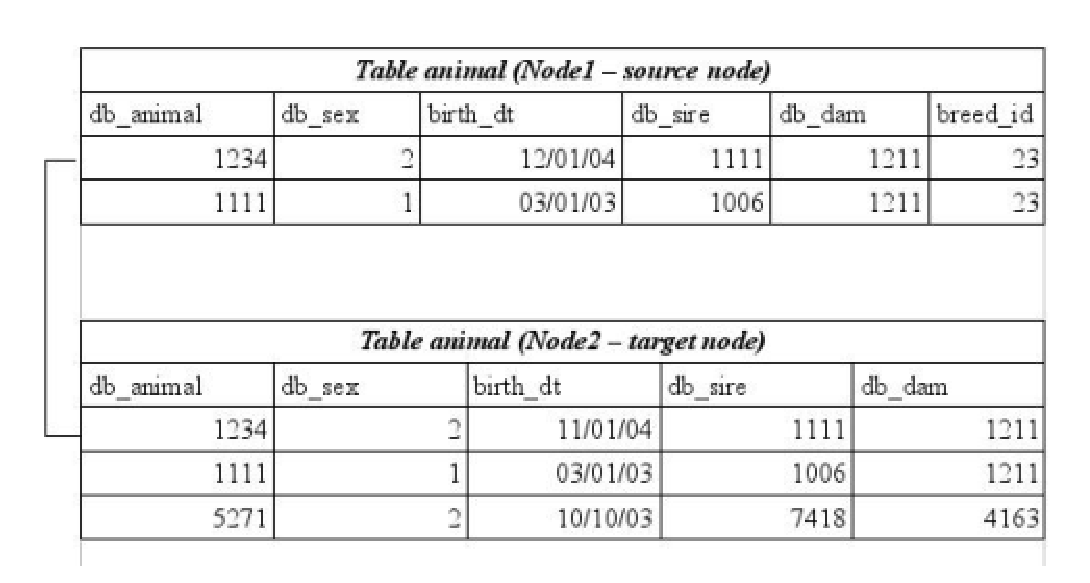
\includegraphics[%
  width=1.0\linewidth]{./synchronization/tables.eps}\end{center}

\begin{center}Information part: (1234,2,12/01/04,1111,1211)\end{center}
\end{figure}
\\
Two nodes can exchange information by setting source/target fields
of the desired data element. For consistency reasons the following
rule should apply: The source field of DE in the receiver node is
the address of the sender node and the target field of the sender
contains the receiver address . \\
This data flow, managed by setting source/target fields is regulated
by Network manager in cooperation with all nodes, thus preventing
inconsistencies in the system.\\
Also, as stated before, only owner can make representative changes
of a data element and this changes are obligatory for all other nodes.

In a generic system there will be three type of nodes:

\begin{itemize}
\item nodes that are only sources of information for the others
\item nodes that are only targets
\item nodes that are sources for some data elements and targets for other
data elements
\end{itemize}
An example of such general animal biodiversity system topology is
shown on Figure \ref{cap:General-system-topology}.%
\begin{figure}

\caption{General system topology\label{cap:General-system-topology}}

\begin{center}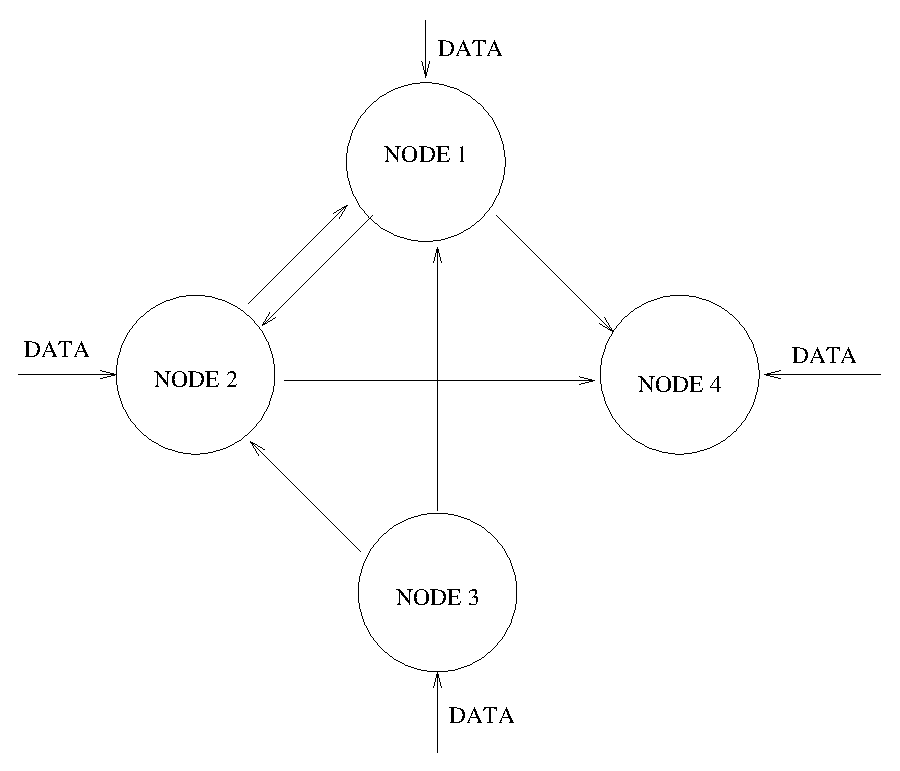
\includegraphics[%
  width=1.0\linewidth,
  keepaspectratio]{./synchronization/univtopology.eps}\end{center}
\end{figure}
 NODE3 is an example of the first kind, NODE4 - of the second and
NODE1 and NODE2 are examples of the third kind. In this example the
content of NODE4 will look like on Figure \ref{cap:NODE4-data-content}.
%
\begin{figure}

\caption{NODE4 data content\label{cap:NODE4-data-content}}

\begin{center}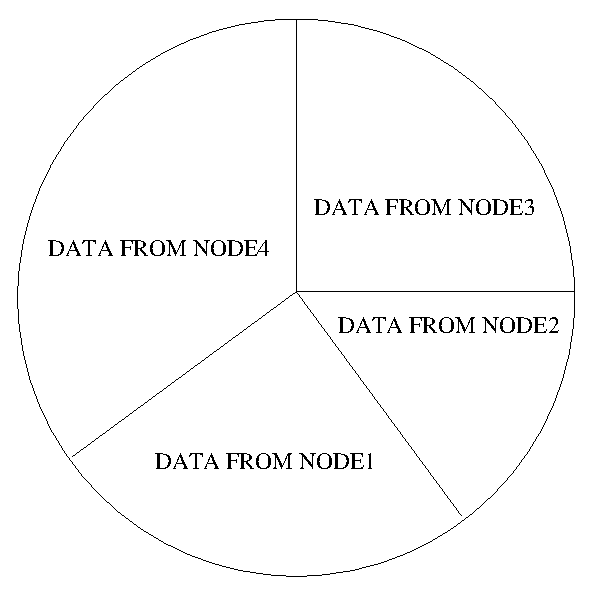
\includegraphics{./synchronization/nodedata.eps}\end{center}
\end{figure}
In the defined above terms {}``Data from NODE3'' means data owned
by NODE3 (initially loaded in NODE3). This data can be received via
NODE1 or NODE2 and the route depends on the source-target pairs. It
is possible that part of the data elements are distributed via NODE1
and part - via NODE2, but it is not possible that one data element
has NODE1 and NODE2 as sources simultaneously.


\section{Functional model}

The functional model of the synchronization process of farm animal
data is shown on Figure \ref{cap:Functional-model}. %
\begin{figure}

\caption{Functional model\label{cap:Functional-model}}

\begin{center}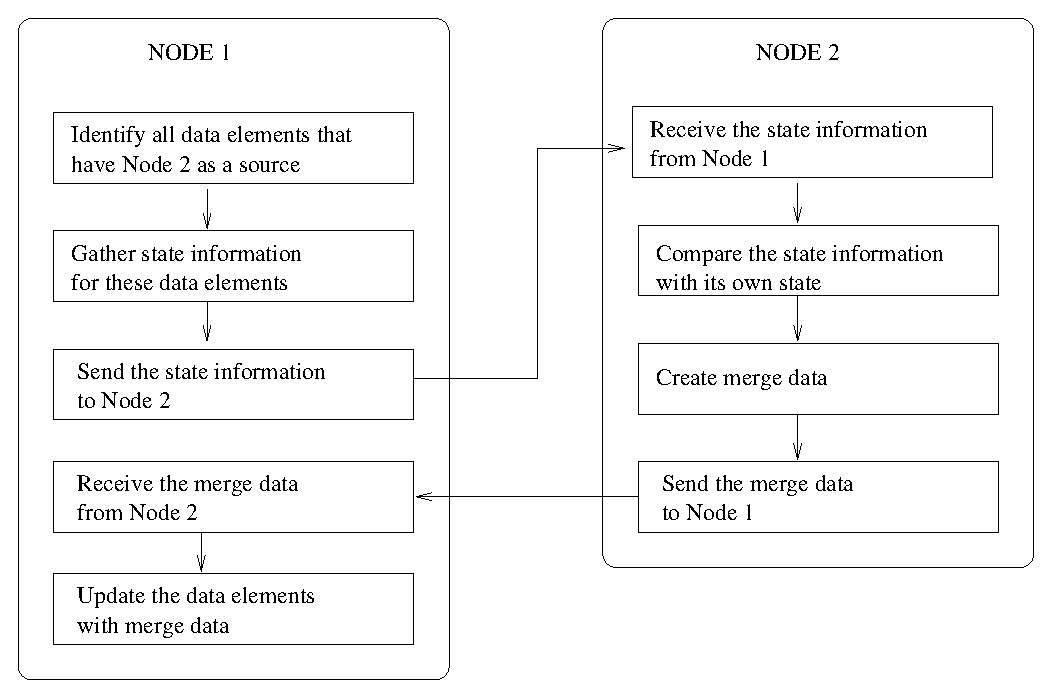
\includegraphics[%
  width=1.0\linewidth]{./synchronization/functmodel.eps}\end{center}
\end{figure}

\section{Implementation}
The implementation has to include the following steps:
\begin{itemize}
\item Setting unique node name\\
Each node has to have unique name within the APIIS-network. THis name is given by the local administrator, but has to be co-ordinated with the Network Manager. The name is set in the local '/etc/apiisrc' file.

\begin{verbatim}
[SYNCHRONISATION]
node_name = EAAP
\end{verbatim} 

\item Setting unique node ip\_address
Each node must have static ip\_address which is accessible from each node within the network. In addition port 5431 has to be open for incomming connections (this is the port where the server daemon listens). The ip\_address is also set in local '/etc/apiisrc' file

\begin{verbatim}
[SYNCHRONISATION]
node_ip = 10.1.1.126
\end{verbatim} 

\item Setting unique numbering interval
Each node in the system has to have unique record numbers and also unique animal internal numbers. The numbering range has to be obtained from from Network Manager and set in local '/etc/apiisrc' file:

\begin{verbatim}
[SYNCHRONISATION]
sequence_interval=1:100000000
\end{verbatim} 

The initialization of all sequence generators is done via the 'CreateDatabase' subroutine. It encapsulates the subroutines: 'LoadNodeData' and 'SetSequences' which are responsible for loading the local nodename and address in the database and setting the numbering interval for all sequences.
\item Setting information about the other nodes in the network
This is done via the program 'nodemanagement.pl' using the menu Settings$>$Nodes.
\item Setting information about the sources
This is done via the program 'nodemanagement.pl' using the menu Settings$>$Sources.
\item Setting information about the targets
This is done via the program 'nodemanagement.pl' using the menu Settings$>$Targets.
\end{itemize}

